% Copy this directory into your paper's figures/ directory.
% Requires \usepackage{graphicx}. Diagnostic pilot; not a benchmark result.
\begin{figure*}[t]
\centering
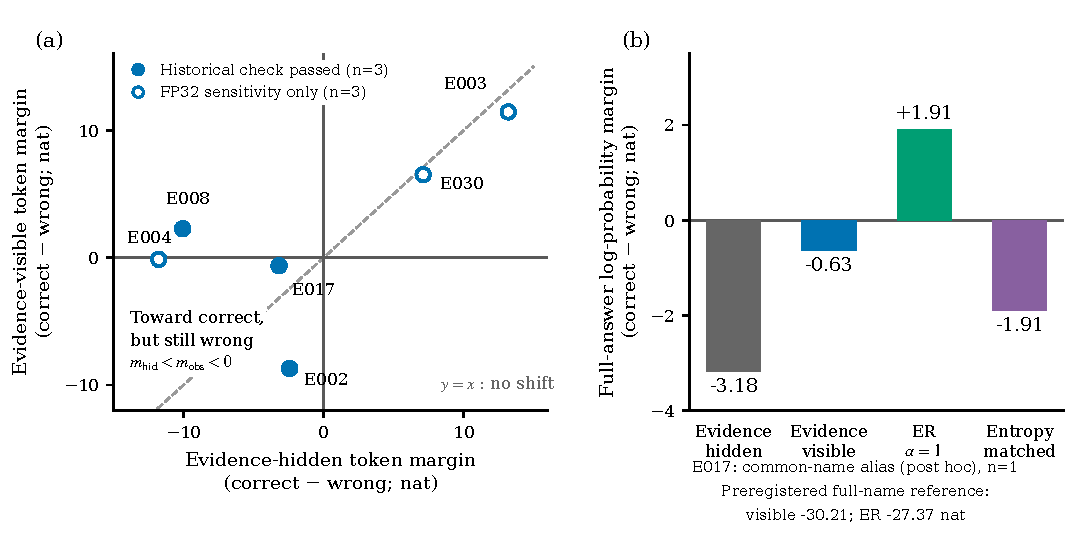
\includegraphics[width=\textwidth]{figures/er_evidence_gap_20260915/evidence_update_gap.pdf}
\caption{\textbf{Making retrieved evidence directly visible can improve correct-candidate support without reversing the teacher target's preference.}
(a) Correct-versus-wrong token log odds at the first divergent token, under the same shared prefix, for all six technically eligible, evidence-sufficient student errors in a frozen diagnostic panel. Seven such semantic errors were found in a 40-case stratified review; one malformed-label case was excluded before fixing the six inputs. Above the diagonal denotes a positive evidence-visibility shift; below the horizontal zero line denotes a remaining wrong-token preference. Filled markers pass the historical log-probability reproduction check; open markers fail that check and are reported only as within-teacher CPU FP32 sensitivity results. E017 and E004 satisfy $m_{\mathrm{hid}}<m_{\mathrm{obs}}<0$; E002 exhibits an adverse shift.
(b) A post-hoc, full-answer alias comparison for E017: ``Ernest Hemingway'' versus ``Elias Canetti,'' including the native closing tokens. The evidence-visible teacher remains wrong in this pairwise ranking; the ER target ($\alpha=1$) reverses it, while a label-free, per-position entropy-matched visible teacher does not. With the preregistered reference ``Ernest Miller Hemingway,'' both the visible and ER full-answer margins remain negative ($-30.21$ and $-27.37$). All evaluations use the same frozen 7B teacher and fixed student histories; masking blocks direct evidence access and does not remove information already carried by those histories. The panels show a local diagnostic and a selected alias sensitivity, not prevalence, decoding accuracy, or student-training gains.}
\label{fig:evidence-update-gap}
\end{figure*}
